\section{Ergebnisse und Evaluation}
\label{sec:ergebnisse}

\subsection{Trainingsverlauf}

\begin{figure}[htbp]
    \centering
    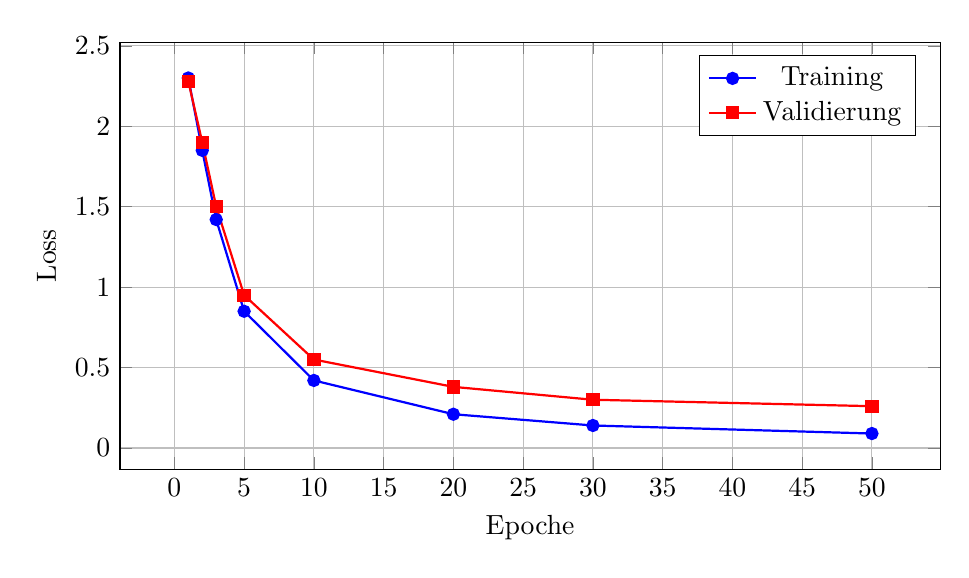
\begin{tikzpicture}
    \begin{axis}[
        xlabel={Epoche}, ylabel={Loss},
        grid=both, width=12cm, height=7cm,
        legend pos=north east,
    ]
    \addplot[blue, thick, mark=*] coordinates {
        (1, 2.30) (2, 1.85) (3, 1.42) (5, 0.85) (10, 0.42) (20, 0.21) (30, 0.14) (50, 0.09)
    };
    \addplot[red, thick, mark=square*] coordinates {
        (1, 2.28) (2, 1.90) (3, 1.50) (5, 0.95) (10, 0.55) (20, 0.38) (30, 0.30) (50, 0.26)
    };
    \legend{Training, Validierung}
    \end{axis}
    \end{tikzpicture}
    \caption{Loss-Verlauf über die Epochen. [DURCH ECHTE DATEN ERSETZEN]}
    \label{fig:loss-verlauf}
\end{figure}

\subsection{Genauigkeit auf dem Testdatensatz}

\begin{hinweisbox}[Platzhalter]
Ergebnisse der Evaluation: Testgenauigkeit, Vergleich mit Trainings- und Validierungsgenauigkeit. Falls Klassifikation: Konfusionsmatrix.
\end{hinweisbox}

\subsection{Fehleranalyse}

\begin{hinweisbox}[Platzhalter]
Beispiele für korrekt und falsch klassifizierte Eingaben. Mögliche Ursachen für Fehler.
\end{hinweisbox}

\subsection{Einfluss der Hyperparameter}

\begin{hinweisbox}[Platzhalter]
Vergleich verschiedener Lernraten, Layer-Größen oder Aktivierungsfunktionen. Welche Konfiguration hat am besten funktioniert?
\end{hinweisbox}

\newpage